% Poster title as heading, author as subheading, supervisor as subsubheading, within the left column
\begin{center}
% Title (bold, centered, 30pt)
\textbf{\Large ILP-Based Delete Relaxation Heuristics for\\\vspace*{2mm}Partial Order Causal Link (POCL) Planning}\\
% Subtitle (bold, centered, 20pt)
\vspace*{2mm}
\textbf{\large Scott Howsam, supervised by Pascal Bercher}\\
\large The Australian National University 
\end{center}
\vspace*{2mm}
\Block{A Problem with POCL Planning}{
\begin{itemize}
	\item Classical state-based planning is an AI problem-solving technique which searches the space of states for an executable sequence of actions which reaches a goal state from an initial state.
    \item In contrast, POCL planning searches the space of partial plans.
    \begin{itemize}
  	    \item A partial plan contains a set of partially ordered actions, and causal links representing causal dependencies between these actions.
  	    \item A causal link protects a precondition by marking an effect as its achiever. Any possible deletion of this effect is a causal threat.
  	    \item A solution to a POCL plan has all preconditions protected by a causal link, and all causal threats resolved.			
    \end{itemize}
    \item Why do POCL planners underperform classical planners?
    \begin{itemize}
		\item While information dense partial plans allow for a compact search space, they also make it difficult to create informed heuristics.
		\item Current POCL heuristics run in polytime by ignoring large amounts of partial plan information, but this is a waste of the work the planner has done to find that information.
  \end{itemize}
\end{itemize}
}

The additive heuristic is state of the art for POCL planning, but ignores most partial plan information. This would be inconceivable in state-based planning. Figure 1 shows the ignored information, and Figure 2 shows how this can lead to inaccurate solutions being considered.
\begin{center}\begin{figure}[ht]
  \centering
  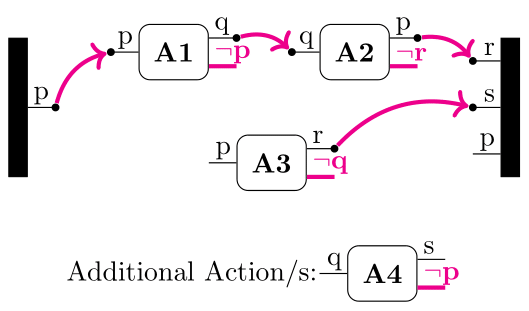
\includegraphics[width=0.8\textwidth]{imgs/new-partial-add.png}
  \caption{A partial POCL plan, with the information relaxed by the additive heuristic in purple. Arrows represent causal links.}
\end{figure}\end{center}
\begin{center}\begin{figure}[ht]
  \centering
  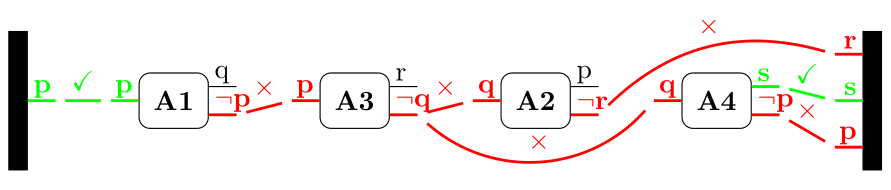
\includegraphics[width=0.95\textwidth]{imgs/new-total-add.png}
  \caption{An inaccurate solution to Figure 1 considered by the additive heuristic. Achieved and unachieved preconditions are marked.}
\end{figure}\end{center}


\Block{A Potential Solution: NP-Hard Heuristics}{
\begin{itemize}
	\item How do we make POCL heuristics more informed? 
	\begin{itemize}
		\item Our heuristic respects all current partial plan information, including causal links. It relaxes the delete-effects of added actions.
		\item This makes it NP-complete, but also more informed, for example it only considers valid solutions to Figure 1.
	\end{itemize}
	\item POCL Planning is PSPACE-complete, so solving it using many NP-complete heuristic calculations could empirically pay out.
\end{itemize}
}

Below is an example of how our heuristic would be calculated on the example partial plan in Figure 3.
\begin{center}\begin{figure}[ht]
  \centering
  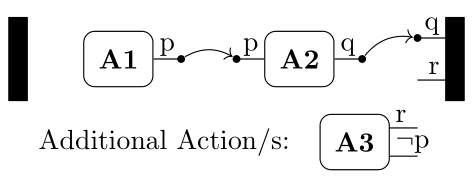
\includegraphics[width=0.8\textwidth]{imgs/new-uncompiled.png}
  \caption{A simple partial POCL plan.}
\end{figure}\end{center}
We first compile the causal links into variables, and then remove the delete effects of actions not already in the partial plan. This can be seen in Figure 4. Note how because of the compilation of causal links, A3 still can't raise a causal threat by being inserted between A1 and A2.
\begin{center}\begin{figure}[ht]
  \centering
  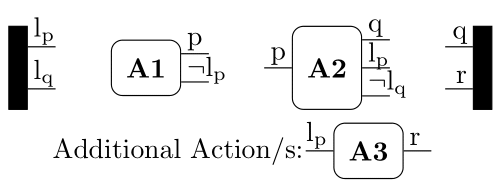
\includegraphics[width=0.9\textwidth]{imgs/new-compiled.png}
  \caption{The relaxation of Figure 3 considered by our heuristic.}
\end{figure}\end{center}
Finally, we translate the relaxed partial plan into an Integer Linear Program (ILP) to solve it. An example optimal solution plan is shown in Figure 5, which would correspond to an optimal solution to the ILP. We later give an example of one of the constraints of the ILP.
\begin{center}\begin{figure}[ht]
  \centering
  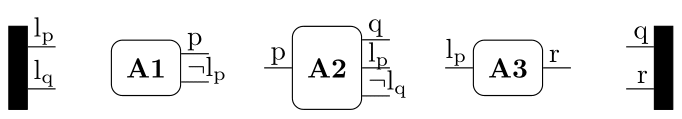
\includegraphics[width=0.95\textwidth]{imgs/new-solved.png}
  \caption{An example optimal solution to Figure 4.}
\end{figure}\end{center}
\Block{ILP Goal Achievement Constraint}{
\begin{itemize}
    \item Here is a simplified goal achievement constraint used in the ILP:
    \[\forall g\in \mathit{Goal}: \sum_{p\in P,p=g}\mathit{Achieved}(p)-\sum_{a\in A,g\in \mathit{Del}(a)}\mathit{Used}(a)\geq 1\]
	\item By comparing the number of times a goal is achieved and deleted, we can ensure that all goals are achieved at the end of the plan.
	\item Other constraints, such as ensuring preconditions are met, additionally utilise time variables for actions and preconditions.
\end{itemize}
}
\Block{Summary of Results}{
\begin{itemize}
    \item Our heuristic is much slower and solves less problems than other heuristics for both feasible and infeasible domains, however it is more informed. The figures below show comparisons to the additive heuristic for IPC2002 problems solved within 10 minutes.
\end{itemize}
}

\begin{center}\begin{figure}[ht]
\centering
\begin{tikzpicture}
\begin{axis}[
	%title={Number of Generated Search Nodes (Log Scale)},
	xlabel style={anchor=north,yshift=-1em},  % Move x-axis label down
	ylabel style={anchor=east,yshift=1.5em,xshift=4.5em},   % Move y-axis label to the left
	xlabel={Delete-Relaxation Heuristic},
	ylabel={Additive Heuristic},
	scale only axis,
	height=10cm,
	width=20cm,
	xmode=log,
    ymode=log,
    xmin=1,
    xmax=1000000,
    ymin=1,
    ymax=1000000
]
\addplot+[
	mark=*,
	mark size=3pt,
	color=black,
	only marks]
table[]
{data/test.dat};
\addplot[black] coordinates {(1,1) (1000000,1000000)};
\end{axis}
\end{tikzpicture}
\caption{Generated nodes comparison, log scale.}
\end{figure}\end{center}
\begin{center}\begin{figure}[ht]
	\centering
	\begin{tikzpicture}
	\begin{axis}[
		%title={Number of Generated Search Nodes (Log Scale)},
		xlabel style={anchor=north,yshift=-1em},  % Move x-axis label down
		ylabel style={anchor=east,yshift=1.5em,xshift=4.5em},   % Move y-axis label to the left
		xlabel={Delete-Relaxation Heuristic (ms)},
		ylabel={Additive Heuristic (ms)},
		scale only axis,
		height=10cm,
		width=20cm,
		xmode=log,
		ymode=log,
		xmin=1,
		xmax=1000000,
		ymin=1,
		ymax=1000000
	]
	\addplot+[
		mark=*,
		mark size=3pt,
		color=black,
		only marks]
	table[]
	{data/runtime.dat};
	\addplot[black] coordinates {(1,1) (1000000,1000000)};
	\end{axis}
	\end{tikzpicture}
	\caption{Runtime comparison, log scale.}
\end{figure}\end{center}

\Block{Conclusion}{
\begin{itemize}
    \item Our results were poor, but given the large difference in how informed our heuristic is, further research is required to conclusively determine whether ILP heuristics have potential for POCL planning. Our report details multiple future research avenues which could improve heuristic runtime.
\end{itemize}
}